\section{Weighted Graphs and Algorithms}
\TODO{Missing parts from second week}

\subsection{Maximal Flows}

\def\dminus{\ensuremath{d^{-}}}
\def\dplus{\ensuremath{d^{+}}}
\def\real{\mathbb{R}}
\def\natural{\mathbb{N}}
\def\Gammaplus{\ensuremath{\Gamma^{+}}}
\def\Gammaminus{\ensuremath{\Gamma^{-}}}

\begin{definition}
\index{flow network}
Let $G=(V,E,w)$ be a directed network with
\begin{compactitem}
\item a weight function $w: E\mapsto \real_0^{+}$,
\item a source $s: \dminus(s) = 0$ and
\item a sink $t: \dplus(t) = 0$.
\end{compactitem}
Then $(V, E, w, s, t)$ is a \dt{flow network}.
\end{definition}

\begin{definition}
\index{flow}
$\phi: E\mapsto \real$ is a \dt{flow} on $G$ if
\begin{align*}
  &\forall e\in E: 0 ≤ \phi(e) ≤ w(e)
     &&\text{feasability condition} \\
  &\forall x\in V\setminus\{s,t\}:
     \underbrace{\sum_{y\in \Gammaminus(x)} \phi(yx)}_{\text{in-flow}} =
     \underbrace{\sum_{y\in \Gammaplus(x)} \phi(xy)}_{\text{out-flow}}
     &&\text{flow conservation condition} \\
\end{align*}
\end{definition}

\begin{definition}
The \dt{size} or \dt{valuation} $v(\phi)$ of $\phi$ is
\[
  v(\phi) = \sum_{y\in \Gammaplus(s)} \phi(sy).
\]
\end{definition}

\TODO{Lemma+Proof out-flow of source = in-flow of sink}

% new content

\begin{definition}
\index{cut!of a flow network}

A partition $V=S \cup T$ ($S\cap T=\varnothing$) such that $s \in S, t \in T$
is called a \dt{cut} of $G$.
\end{definition}

\begin{definition}
\index{capacity!of a cut}
The \dt{capacity} $c(S,T)$ of a cut is given by
\[ c(S,T) = \sum_{x\in S, y\in T} w(xy). \]
\end{definition}

A cut $(S,T)$ is minimal if all cuts $(S',T')$ satisfy $c(S', T') \geq c(S,T)$.

\Lemma. Let $G$ flow network, $\phi$ flow on $G$, $(S,T)$ cut of G. Then
\[
v(\phi) = \underbrace{\sum_{x\in S, y\in T} \phi(xy)}_{\text{flow forward}}
        - \underbrace{\sum_{x\in T, y\in S} \phi(xy)}_{\text{flow backwards}}
\leq c(S,T).
\]
In particular,
\[
  \max_{\text{flow $\phi$}} v(\phi)\leq \min_{\text{cut $(S,T)$}} c(S,T).
\]

\Proof.
\[
    v(\phi) = \sum_{v\in S} \left(
        \sum_{x\in \Gamma^+(v)} \phi(vx)
      - \sum_{y\in \Gamma^-(v)} \phi(yv)
    \right)
\]

For each vertex, we count flow on outgoing edges positive and flow on
incoming edges negative. We have the following cases:
\begin{itemize}
  \item Flow with both endpoints in $S$; outgoing and ingoing cancel each other
  \item Flow with starting point in $S$ and end point in $T$, counted positive
  \item Flow with starting point in $T$ and end point in $S$, counted negative
\end{itemize}

\begin{figure}[htb]
  \centering
  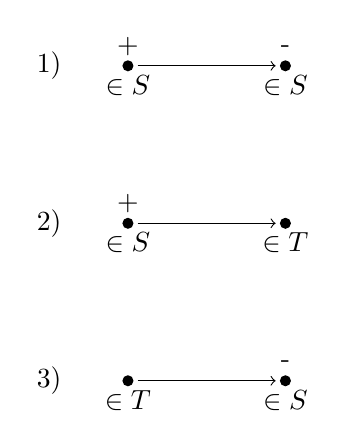
\begin{tikzpicture}
    \node (a0) at (0,0) {1)};
    \node (a1) at (1,0) {};
    \node (a2) at (3,0) {};
    \node (b0) at (0,-2) {2)};
    \node (b1) at (1,-2) {};
    \node (b2) at (3,-2) {};
    \node (c0) at (0,-4) {3)};
    \node (c1) at (1,-4) {};
    \node (c2) at (3,-4) {};
    
    \node at (1,0.25) {+};
    \node at (3,0.25) {-};
    \node at (1,-2 +0.25) {+};
    \node at (3,-4 +0.25) {-};
  
    \node at (1,-0.25) {$\in S$};
    \node at (3,-0.25) {$\in S$};
    \node at (1,-2.25) {$\in S$};
    \node at (3,-2.25) {$\in T$};
    \node at (1,-4.25) {$\in T$};
    \node at (3,-4.25) {$\in S$};
  
    \def\numone{1}
    \def\numtwo{2}
    \foreach \node in {a,b,c} 
    {
      \fill (\node\numone) circle(2pt);
      \fill (\node\numtwo) circle(2pt);
      \path (\node\numone) edge[->] (\node\numtwo);
    };
    
  \end{tikzpicture}
  \caption{3 possible cases}
\end{figure}


Thus, we can rewrite $v(\phi)$:
\[
    v(\phi) = \sum_{x\in S, y\in T} \phi(xy)
            - \sum_{x\in T, y\in S} \phi(xy)
\]
Observe that in the first sum, all $\phi (xy) \leq w(xy)$. The second sum is
nonnegative: $0 \leq \phi (xy) \leq c(S,T)$.

Thus
\[
    v(\phi) \leq c(S,T).
\]

\begin{definition}
\index{augmenting path}
A path $P: s\rightarrow t$ (ignoring edge direction) is said to be an \dt{augmenting
path} with respect to a flow $\phi$ if $\phi(e) < w(e)$ on every forward edge
of $P$ and $\phi(e) > 0$ on every backward edge.
\end{definition}

\textbf{Theorem.}
Let $G$ flow network, $\phi$ flow on $G$. Then 
\[v(\phi)\text{ maximal} \iff \nexists\text{ augmenting path (w.r.t. $\phi$)}.\]

\ProofForward.
Suppose there is an augmenting path $P$. Then we choose
\begin{alignat*}{3}
    \delta' &= \min_{e \in P,\text{ forward}} w(e) - \phi(e) &\null> 0 \\
    \delta'' &= \min_{e\in P,\text{ backward}} \phi(e) &\null> 0 \\
    \delta &= \min(\delta', \delta'') &> 0
\end{alignat*}

Define
\[
    \tilde\phi := \begin{cases}
        \phi(e) + \delta &\text{if $e$ forward edge of $P$} \\
        \phi(e) - \delta &\text{if $e$ backward edge of $P$} \\
        \phi(e) &\text{otherwise}.
    \end{cases}
\]

$\tilde\phi$ is a flow on $G$.

Because we take the minimum of all the flows $\delta$, $\tilde\phi$ does not become negative on backward edges.

Because we increase the flow on the augmenting path by $\delta$,
\[
    v(\tilde\phi) = v(\phi) + \delta > v(\phi).
\]

\ProofBackward.
Assume there is no augmenting path. Let
\[
    S = \{v\in V \mid \exists\;\text{augmenting path $s\rightarrow v$}\}.
\]
There is no augmenting path $s\rightarrow t$, thus $t \notin S$.
Thus $(S, T = V\setminus S)$ is a cut.
Each edge $xy$ with $x\in S, y\in T$ must be saturated: otherwise it would be possible to find an augmenting path.

\begin{figure}[htb]
  \centering
  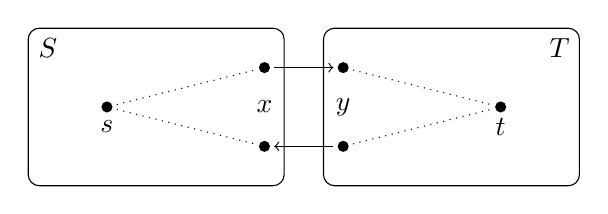
\begin{tikzpicture}
    \node (s) at (2,2) {};
    \node (x1) at (4,2.5) {};
    \node (x2) at (4,1.5) {};
    \node (y1) at (5,2.5) {};
    \node (y2) at (5,1.5) {};
    \node (t) at (7,2) {};
  
    \node at (2,1.75) {$s$};
    \node at (7,1.75) {$t$};
    \node at (4,2) {$x$};
    \node at (5,2) {$y$};
  
    \foreach \node in {s,x1,x2,y1,y2,t}
    {
      \fill (\node) circle(2pt);
    };
    \path (x1) edge[->] (y1);
    \path (y2) edge[->] (x2);

    \path[dotted] (s) edge (x1);
    \path[dotted] (s) edge (x2);
    \path[dotted] (y1) edge (t);
    \path[dotted] (y2) edge (t);

    \node (S) at (1.25,2.75) {$S$};
    \node (T) at (7.75,2.75) {$T$};
    \draw[rounded corners] (1,1) rectangle (4.25,3);
    \draw[rounded corners] (4.75,1) rectangle (8,3);
  \end{tikzpicture}
  \caption{Proof augmented path}
\end{figure}



Each edge $xy$ with $x\in T, y\in S$ must be void ($\phi(xy) = 0$). Thus
\[
    v(\phi) = c(S,T) - 0.
\]

Therefore $\phi$ must be maximal.

\textbf{Theorem.} If $G$ is a flow network such that $\forall e\in E': w(e)\in
\mathbb{N}$, a maximal flow exists.

\textbf{Proof.} $ \phi_{0}(e) \equiv 0$, if $\phi_{0}$ not max $\implies \exists$ augmenting path with $\delta \in \mathbb{N^{+}}$

Construct $\phi_1$ according to previous proof ($\tilde\phi$). We know that $v(\phi_1) ≥ 1$. Now we iterate and get $\phi_2, v(\phi_2) ≥ 2$,~\ldots After finitely many steps, we reach a flow $\phi_{\text{max}}$ where we cannot find an augmenting path anymore.

\textbf{Corollary.} If $G$ is a flow network with a weight function $w: E\mapsto \mathbb{Q}$, this implies $\exists\;\text{maximal flow}$.

\textbf{Remark.}
If weights are real, it can also be shown that a maximal flow exists (but you need a different proof strategy).

\textbf{Theorem (Max-flow/min-cut theorem).}
Let $G$ be a flow network $\implies \exists$ max. flow and $v(\phi_{\text{max}})= \min_{(S,T) cut} c(S,T)$

% slides: Algorithm of Ford-Fulkerson
